\subsubsection{Self-Similar infall test}
\label{sec.tests.infall}

The next test problem is based on the self-similar solutions to the cosmological spherical infall problem found by \citet{Bertschinger1985}.  It features a small density perturbation in a homogeneous $\Omega = 1$ universe and is a strong test of the cosmological evolution, gravity, and hydrodynamic portions of the code.  It is close analogue to cosmological cluster formation and has an analytic solution.

For initial conditions, we adopt a $32^3$ top grid with a single, initial sub grid (covering $1/8^3$ of the domain) with a refinement factor of 2.  An overdensity $\delta = 40$ is placed in a single cell near the center of the domain.  We begin at $z=199$ and evolve to $z=0$, which is a sufficient time for the evolution to largely forget its initial conditions and approach the self-similar result.  An over density refinement criteria ($\delta_{\rm crit} = 1.1$ on the top grid) is used to add additional grids, going up to 5 additional levels beyond the root grid.  We use the PPM solver without radiative cooling; only baryons are used for this problem.  An ideal gas law with $\gamma = 5/3$ is adopted.

In Figure~\ref{fig.sphericalinfall}, we show the results, scaled according to the dimensionless variables as defined in equations (2.9) and (3.2) of \citet{Bertschinger1985}.  This demonstrates that we can quickly and easily obtain a good solution with only a fairly modest initial grid.  The shock is sharply resolved and the asymptotic profiles as small $\lambda$ are recovered.  At very small values of $\lambda$, the initial conditions have not been fully forgotten and the self-similar solution is not recovered -- this can be seen most clearly in the dimensionless mass; however, this is simply because of the limited amount of time for which we evolved the solution.


\begin{figure}
\begin{center}
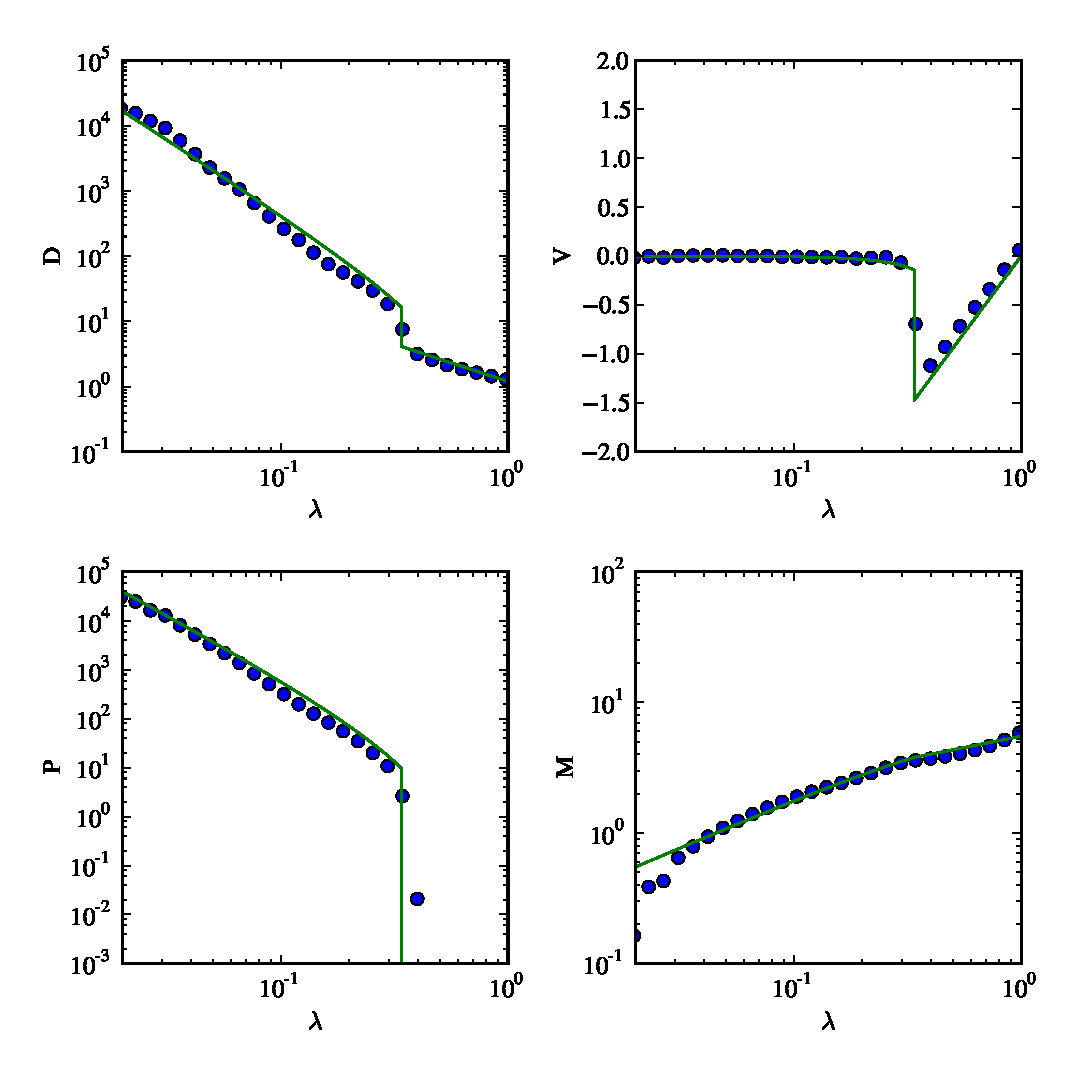
\includegraphics[width=0.7\textwidth]{figures/SphericalInfall.eps}
\caption{The results of the self-similar spherical infall test.  The panels show, as a function of the dimensionless radius $\lambda$, the dimensionless density $D$ (top left), velocity $V$ (top right), pressure $P$ (bottom left), and enclose mass $M$ (bottom right).  In each case we show azimuthally averaged profiles from the simulation as circles and the analytic solution for for $\gamma = 5/3$ as solid lines.}
\label{fig.sphericalinfall}
\end{center}
\end{figure}